\documentclass[graphics]{beamer}

\usepackage{graphicx}
\usepackage{verbatim}
\usepackage{wrapfig}
\useoutertheme{shadow}
%\usecolortheme{orchid}
\usecolortheme{seahorse}


% math commands
\newcommand{\be}{\begin{eqnarray}}
\newcommand{\ee}{\end{eqnarray}}
\newcommand{\beq}{\begin{equation}}
\newcommand{\eeq}{\end{equation}}
\def\simless{\mathbin{\lower 3pt\hbox
      {$\rlap{\raise 5pt\hbox{$\char'074$}}\mathchar"7218$}}}
\def\simgreat{\mathbin{\lower 3pt\hbox
      {$\rlap{\raise 5pt\hbox{$\char'076$}}\mathchar"7218$}}} %> or of order

% variables

\def\toonscale{0.45}
\def\mboxy#1{\mbox{\small #1}}


\begin{comment}
\AtBeginSection[]{
  \frame{
    \frametitle{Outline}
    \tableofcontents[currentsection]
  }
}
\end{comment}

\title{Science with a billion IM modes
}
\subtitle{}
\author[U. Pen]{\textcolor{green}{Ue-Li Pen
}
\\[8mm] 
}
\date{February 21, 2019}


\begin{document}

\frame{
\begin{picture}(320,250)
\put(-30,-110){
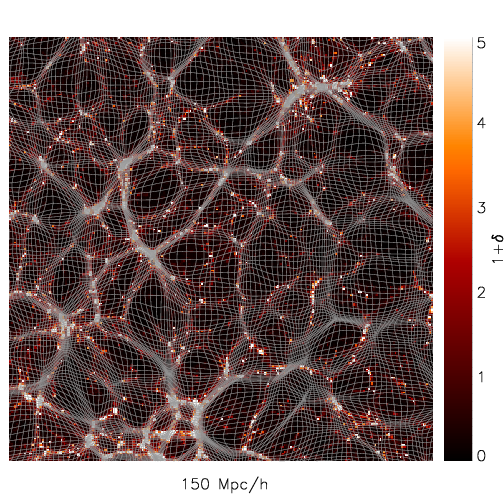
\includegraphics[width=5.5in]{Figures/map0512-0128_i1500_.png}}
\end{picture}
\vspace{-3in}
\titlepage
}

%\section*{Introduction}


\begin{comment}
  \subsection{Outline}

  \frame{
    \frametitle{Outline}
    \tableofcontents
  }
\end{comment}

\section{Mode counting}
  \frame{
\vspace{-0.5in}
    \frametitle{Saturation}
    \begin{itemize}
      \item Eulerian density decorrelated from initial conditions for $k>0.1h$/Mpc
      \item Eulerian Fisher information saturates at $k>0.1h$/Mpc
      \item Universe near Eulerian 'cosmic variance' after current
        generation of surveys (DESI)
     \end{itemize}
  }

  \frame{
\vspace{-0.5in}
    \frametitle{non-Linear Reconstruction}
    \begin{itemize}
      \item similar performance confirmed by several groups (Nanjing,
        Toronto, Princeton, Durham, Paris) 
      \item recovers linear Lagrangian modes and phases out to $k\sim 1h$/Mpc
      \item 1000x more information than Eulerian, $\sim 10^9$ modes
      \item still biased tracers: need to marginalize over bias, etc.
      \item BAO: 4x info increase (Wang et al 2017)
      \item New theory needed: RSD, bispectrum, etc
     \end{itemize}
  }

\frame{
    \frametitle{3-D: E-mode}
%\vspace{-0.5in}
\hspace{-0.2in}\includegraphics[width=2.3in]{Figures/nonlinear.png}  
\vspace{0.15in}\includegraphics[width=2.21in]{Figures/reconstructed.png}  

(from Yu+ 2017, PRD 95, 043501)
  }

  \frame{
    \frametitle{Multigrid solution}
\center{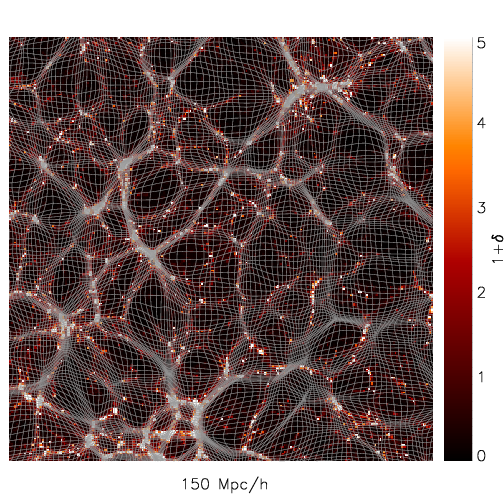
\includegraphics[width=3.0in]{Figures/map0512-0128_i1500_.png}}
{\tiny Zhu++ 2017, PRD, 96, 13502}
}

  \frame{
    \frametitle{Low noise limit}
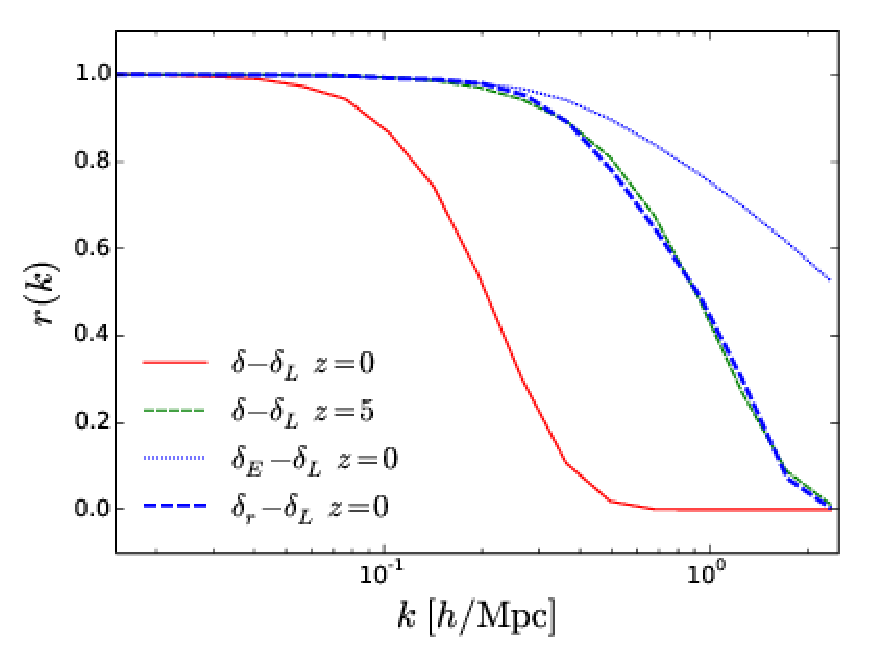
\includegraphics[width=3.4in]{Figures/rk.pdf}
}
  \frame{
    \frametitle{BAO}
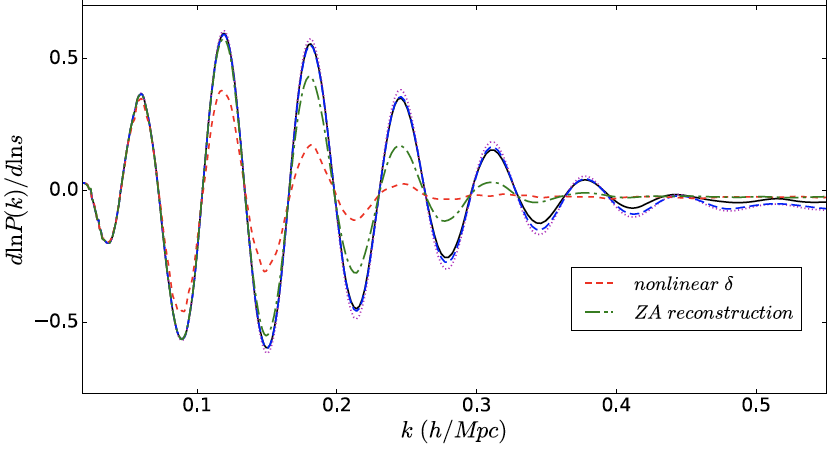
\includegraphics[width=3.4in]{Figures/bao-rec.png}

}
  \frame{
    \frametitle{FoM}
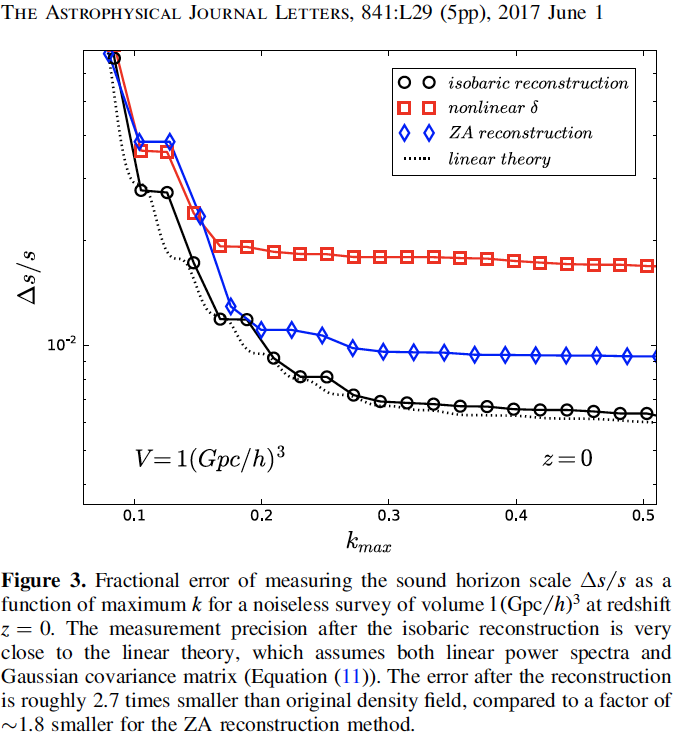
\includegraphics[width=3.4in]{Figures/bao-nl.png}

}

  \frame{
\vspace{-0.5in}
    \frametitle{Physical targets}
    \begin{itemize}
        \item dark energy: low-z anchor
        \item neutrinos: new non-Gaussian theory needed.
        \item CDM gravitational interactions very local: $\sim 1$Mpc
        \item $\nu$'s come from tens of Mpc, carry different
          information: linear momentum, tide, etc.
        \item starting points: CDM-$\nu$ dipole (Zhu++ 2014), dynamical friction
          (Okoli+2017), differential condensation, angular momentum
          (Yu+ 2018)
        \item common (a-)symmetry: squeezed dipole bispectrum
     \end{itemize}
  }

  \frame{
\vspace{-0.5in}
    \frametitle{beyond cosmic variance}
    \begin{itemize}
        \item $\nu$ detection primarily from scale dependent rate of growth
        \item typically uses measurement at two redshifts in two
          different places
        \item think of archeology
     \end{itemize}
  }


\frame{
\vspace{-0.5in}
    \frametitle{Conclusions}
    \begin{itemize}
        \item non-linear reconstruction: 1000x more initial modes than eulerian
        \item statistical power better than $10^{-4}$
        \item disentangle dynamics from gastrophysics
     \end{itemize}
  }


\end{document}
